\section{Evaluation}

\subsection{Experiment Setup}
For our initial evaluation/experimentation, we use Emulab \cite{emulab}. Emulab gives us the ability to configure arbitrary network topologies and link bandwidths. For a start, each node in our Emulab topology acts as a datacenter and a link connecting two nodes will act as a link in the WAN. We have configured our environment in Emulab by installing Spark and its dependencies.  Below we show the results from running `word count' on an emulab cluster containing two connected nodes with traffic-shaping on the link. Our dataset is a subset of wikipedia articles, of size 1GB. We split the dataset into two halves and store each half at each node's local storage. The total number of Map tasks run was 48, while the total number of Reduce tasks was 8. 

Note that Spark requires the data to be stored on a shared filesystem, such as HDFS. To give our system this illusion while ensuring that data is accessed over the traffic-shaped link , we set up NFS servers at each node and disabled client-side caching. Each emulab node has 2GB RAM, and two Intel Xeon 3.00GHz processors.

\subsection{Overall Job Time}
Figure~\ref{fig:job-time} shows how the job execution time changes as the link bandwidth is varied. This is compared against both nodes col-located, i.e., without communication over the WAN. Each data point is the mean of three runs. It clearly shows that the job runtime is very sensitive to the amount of available bandwidth between workers. The job runtime is improved by almost 100 secs when the available bandwidth is increased from 5 to 10 Mbps, with it approaching the runtime for co-located nodes as the bandwidth is increased even further.  

Next, we instrument the Map and Reduce stages of the job independently.

\begin{figure}[!ht]
\centering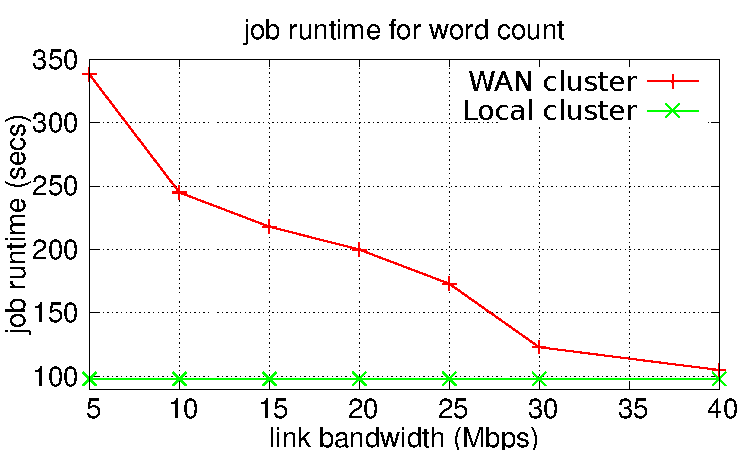
\includegraphics[width=\columnwidth]{figs/job-time.pdf}
\vspace{-1.2em}
\caption{Spark job execution time increases drastically as the wide area link bandwidth decreases.}
\label{fig:job-time}
\vspace{.7em}
\end{figure}

\subsection{Map Statistics}

Figure~\ref{fig:map-time} considers only the map tasks that fetch their data partition remotely. Note that the Map runtime includes the time to fetch the input data partition. It shows how the median runtime decreases almost exponentially as the link bandwidth is increased. Clearly there is a need to avoid these remote fetches
by preventing scheduling of map tasks on remote nodes. 
%An interesting observation is that the number of Map tasks fetching remote input decreases as the bandwidth goes down. This is a result of opportunistic scheduling in Spark since a new map task is scheduled on a core only when the previous one finishes.

\begin{figure}[!ht]
\centering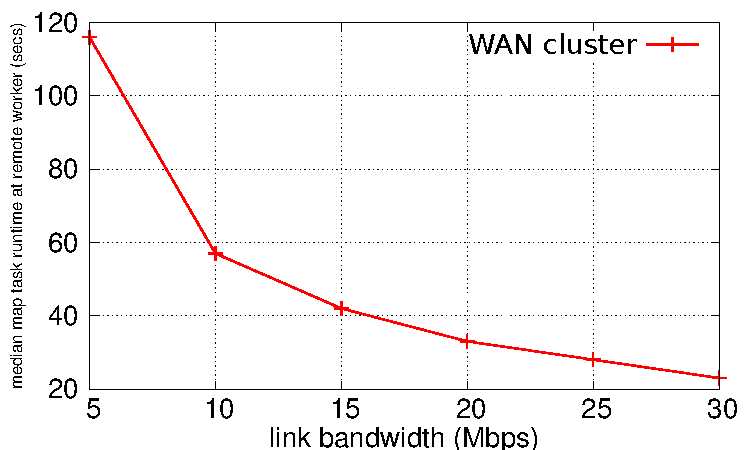
\includegraphics[width=\columnwidth]{figs/map-time.pdf}
\vspace{-1.2em}
\caption{The median execution execution time for a map task that fetches data remotely increases drastically as the wide area link bandwidth decreases.}
\label{fig:map-time}
\vspace{.7em}
\end{figure}

\subsection{Reduce Statistics}

In MapReduce and Shark, a reduce task has to fetch $M$ shuffle blocks. Some of these blocks will be local, while the rest will have to be fetched from remote nodes.  Figure~\ref{fig:reduce-blocks} shows, for each node, how the median number of remote shuffle blocks fetched by reduce tasks changes as the link bandwidth is varied. Here we see that low bandwidth causes a significant discrepancy between the number of shuffle blocks fetched remotely by the two nodes. As the bandwidth is increased, this discrepancy goes down. A higher number of remote shuffle blocks to be fetched by the reducers increases the latency, as shown in Figure~\ref{fig:reduce-time}. We see that because the reduce tasks at node 1 had to fetch a significantly higher number of shuffle blocks remotely, the median reduce runtime for node 1 is higher than node 2.   

\begin{figure}[ht]
	\centering
	\begin{minipage}[b]{0.48\linewidth}
		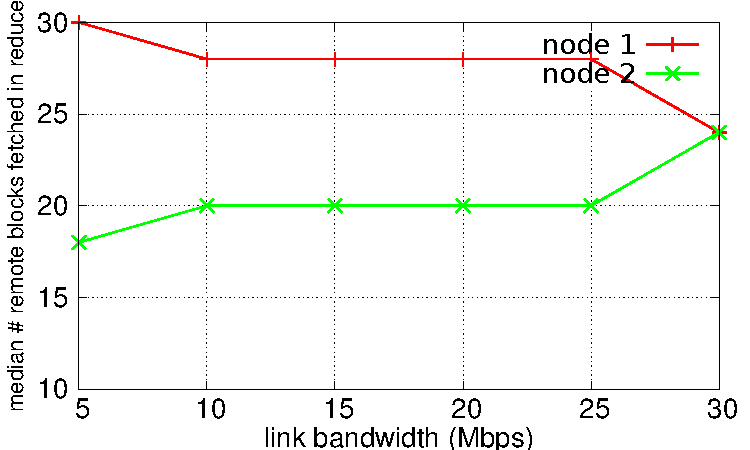
\includegraphics[width=2.5in]{figs/reduce-blocks.pdf}
		\caption{}
		\label{fig:reduce-blocks}
	\end{minipage}
	\quad
	\begin{minipage}[b]{0.48\linewidth}
		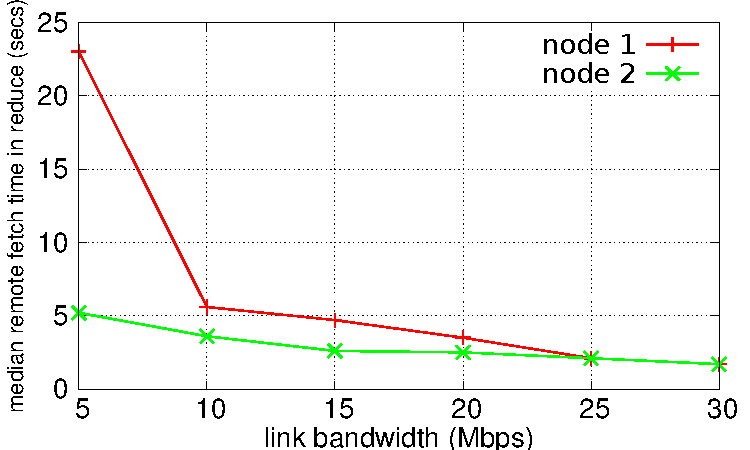
\includegraphics[width=2.5in]{figs/reduce-time.pdf}
		\caption{}
		\label{fig:reduce-time}
	\end{minipage}
\end{figure}

\subsection{Next Steps}

Our next steps are:

\begin{itemize}
\item Flesh out our designed improvements to Spark/MapReduce. As mentioned earlier, this will have two components:
\begin{itemize}
\item Run map tasks only on partitions local to a node. In other words, the Spark job is told which file resides at what node. The scheduler will then need to be modified such that each map is scheduled only for a local partition.
\item    
\end{itemize} Have a sampling-based approach for fetching shuffle blocks in reduce tasks. Note that a reduce task will have to fetch a shuffle block from each map's location. Fetching all these blocks would incur a lot of overhead. Instead we plan to implement and evaluate a sampling-based approach.
\item Implement the operators needed for our case-studies.
\end{itemize}

For a specific query, we envision our result graphs to be like this:

\begin{figure}[ht]
	\centering
	\begin{minipage}[b]{0.48\linewidth}
		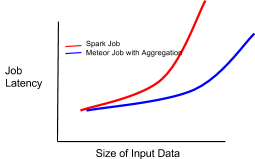
\includegraphics[width=2.5in]{figs/fig_1.png}
		\caption{Latency}
		\label{fig:minipage1}
	\end{minipage}
	\quad
	\begin{minipage}[b]{0.48\linewidth}
		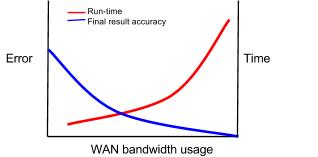
\includegraphics[width=2.5in]{figs/fig_2.png}
		\caption{Error}
		\label{fig:minipage2}
	\end{minipage}
\end{figure}

Here we increase the size of the input data on the x-axis. A Spark job with no topological awareness starts taking longer and longer since the WAN link gets saturated. On the other hand, the corresponding Meteor job takes a lot less time since it uses aggregation to reduce the data needed to be sent over the WAN link. We plan to explore how modulating the bandwidth usage over WAN affects run-time as well as final result accuracy. We expect those result to be highly dependent on the application we are targeting.